\IEEEraisesectionheading{\section{简介}
\label{sec:introduction}}

目标跟踪是计算机视觉领域的重要研究方向之一,其目标是在连续的图像中对感兴趣物体进行检测、提取、识别和跟踪,从而获得目标物体的相关参数,如位置、速度、尺度、轨迹等,并对其进一步处理和分析,实现对目标物体的行为理解,或完成更高一级的任务。

目标跟踪技术有一些典型的应用场景,包括 a)安全监控:车站、机场、银行及超市等公共 场所的实时监控;b)交通检测:对行人及车辆行为进行判定,完善智能交通系统;c)军事领域:导弹制导、武器观测瞄准、敌方目标定位及跟踪;d)医学应用:标记、增强及跟踪生物特征来帮助医生诊断疾病;等。

虽然目标跟踪技术在很多领域都有着广泛的应用前景,但由于实际环境复杂多变,目标跟踪技术也面临着诸多挑战,如光照、尺寸的变化,目标的快速运动,形变,相机抖动,遮挡等复杂的因素。而一个好的目标跟踪算法,应该是要又快又准。“快”主要表现在计算量小和所需的存储空间小,“准”就是在复杂因素的干扰下,预测出的目标位置(bonding box)要尽可能地接近真实值。按照模式划分,目标跟踪的方法可以分为2类,即生成式模型和鉴别式模型。

 早期的工作主要集中于生成式模型跟踪算法的研究, 如光流法、粒子滤波、Meanshift算法、Camshift算法等。这类方法首先建立目标模型或者提取目标特征, 在后续帧中进行相似特征搜索,逐步迭代实现目标定位。但是这类方法也存在明显的缺点, 就是图像的背景信息没有得到全面的利用,且目标本身的外观变化有随机性和多样性的特点, 因而通过单一的数学模型描述待跟踪目标具有很大的局限性。例如在光照变化, 运动模糊, 分辨率低, 目标旋转形变等情况下, 模型的建立会受到巨大的影响, 从而影响跟踪的准确性。

\begin{figure}[!ht]
  \centering
  \begin{minipage}[b]{\linewidth} 
  \subfloat[]{
    \begin{minipage}[b]{0.5\linewidth} 
      \centering
      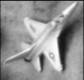
\includegraphics[width=\linewidth]{fig1_a}
       \end{minipage}
  }
  \subfloat[]{
    \begin{minipage}[b]{0.5\linewidth} 
      \centering
      
\includegraphics[width=\linewidth]{fig1_b}
       \end{minipage}
  }
  \end{minipage}
  \vfill
  \caption{目标跟踪示例:(a) 初始化第1帧目标状态, (b) 预测第N帧目标状态.}
  \label{fig:tracker_example}
\end{figure}

鉴别式模型是指将目标模型和背景信息同时考虑在内, 通过对比目标模型和背景信息的差异, 将目标模型提取出来, 从而得到当前帧中的目标位置。一些研究对跟踪算法的评估中发现, 通过将背景信息引入跟踪模型, 可以很好地实现目标跟踪。因此研究人员逐渐尝试使用经典的机器学习方法训练分类器, 如 MIL、TLD、支持向量机等。近年来, 随着深度学习技术的广泛应用, 人们开始将深度学习技术用于目标跟踪,并取得了更加显著的性能。

本文分别在两个视频序列上实现了一种生成式模型跟踪算法和一种鉴别式模型跟踪算法,即基于 Mean Shift 的目标跟踪基于分类思想的目标跟踪。本文剩余部分将对两种目标跟踪方法的原理、实现及实验进行介绍,所有实验涉及的方法、函数实现均基于 Python 语言。